\chapter{Future Development Of Project}
\label{ch:Future_Development_Of_Project}
Now that the \textit{Swing} design has been detailed and expanded, there are only several steps required to make this design a reality.
In this chapter, the future of the \textit{Swing} project is expanded upon.
First and foremost, a development logic diagram shall be created.
Based on this diagram, a detailed Gantt Chart is constructed.

\section{Design and Development Logic}
This section presents the design and development logic for the future.
Based on the flow diagram showcased in \Cref{fig:dev_logic}, it can be seen that there are nine more steps that have to be finalised before the design reaches maturity.
The first step that has to be performed is the finalisation of the detailed aircraft design .
This has to be done taking into account the requirements that have not yet been complied with, as described in \Cref{ch:Requirements_Compliance}.
Thus, the wind gust performance, especially during the hover phase, should be analysed, as well as the roll performance and the hinge design.

After the conceptual design is completed, it is crucial that the team ensures that there is sufficient financial backing in order to achieve success.
This can be achieved through the promotion of the design to different operators, as well as negotiations with different potential investors.

An example of a desired investor for the \textit{Swing eVTOL} project would be an airline company such as KLM.
A crucial marketing aspect of the \textit{Swing eVTOL} design is the fact
that the design is a great solution for the \enquote*{last-mile problem}.
Therefore,
the design can be marketed as a feeder system for the airlines to take VIP passengers
and bring them to the aircraft in a quicker and more efficient way.
This would enable picking passengers up from the city centre of Amsterdam
and bringing them to the airport within half an hour, avoiding traffic and the hustle of public transport.
Another positive aspect of the design is that it would enable KLM
to compete with companies such as NS on the short-haul segment of business passengers.
Therefore,
there are plenty of reasons
why an airline such as KLM would be persuaded to ensure financial backing for the \textit{Swing} project.

With the financial backing ensured, the prototype of the design should be produced and then tested, in order to reach certified status.
Once certification of the design is ensured, the design should be marketed to different operators.
This would enable the start of mass production, which would lead to commercial operation commencement.
Lastly, customer support should be provided by the manufacturer to the customers to achieve a successful end product.

Based on the aforementioned considerations, the project development logic diagram was constructed and is showcased in more detail in \Cref{fig:dev_logic}.
It is important to note that the diagram has three layers of detail.
More detail is presented in the first layers due to closer proximity to the current state of the project and thus a more clear overview of the required steps left to be taken, especially when considering finalising the design.

\section{Gantt Chart}
\label{sec:PostDSE_Gantt_Chart}
After the future steps that have to be taken for the project have been expanded upon, a more detailed Gantt Chart can be provided.
This shall contain all
the relevant tasks that are yet to be performed, along with the responsible person and the expected number of hours.
The Gantt Chart is showcased in the Appendix.

\label{sec:Design_and_Development_Logic} 
\begin{figure}[H]
    \centering
    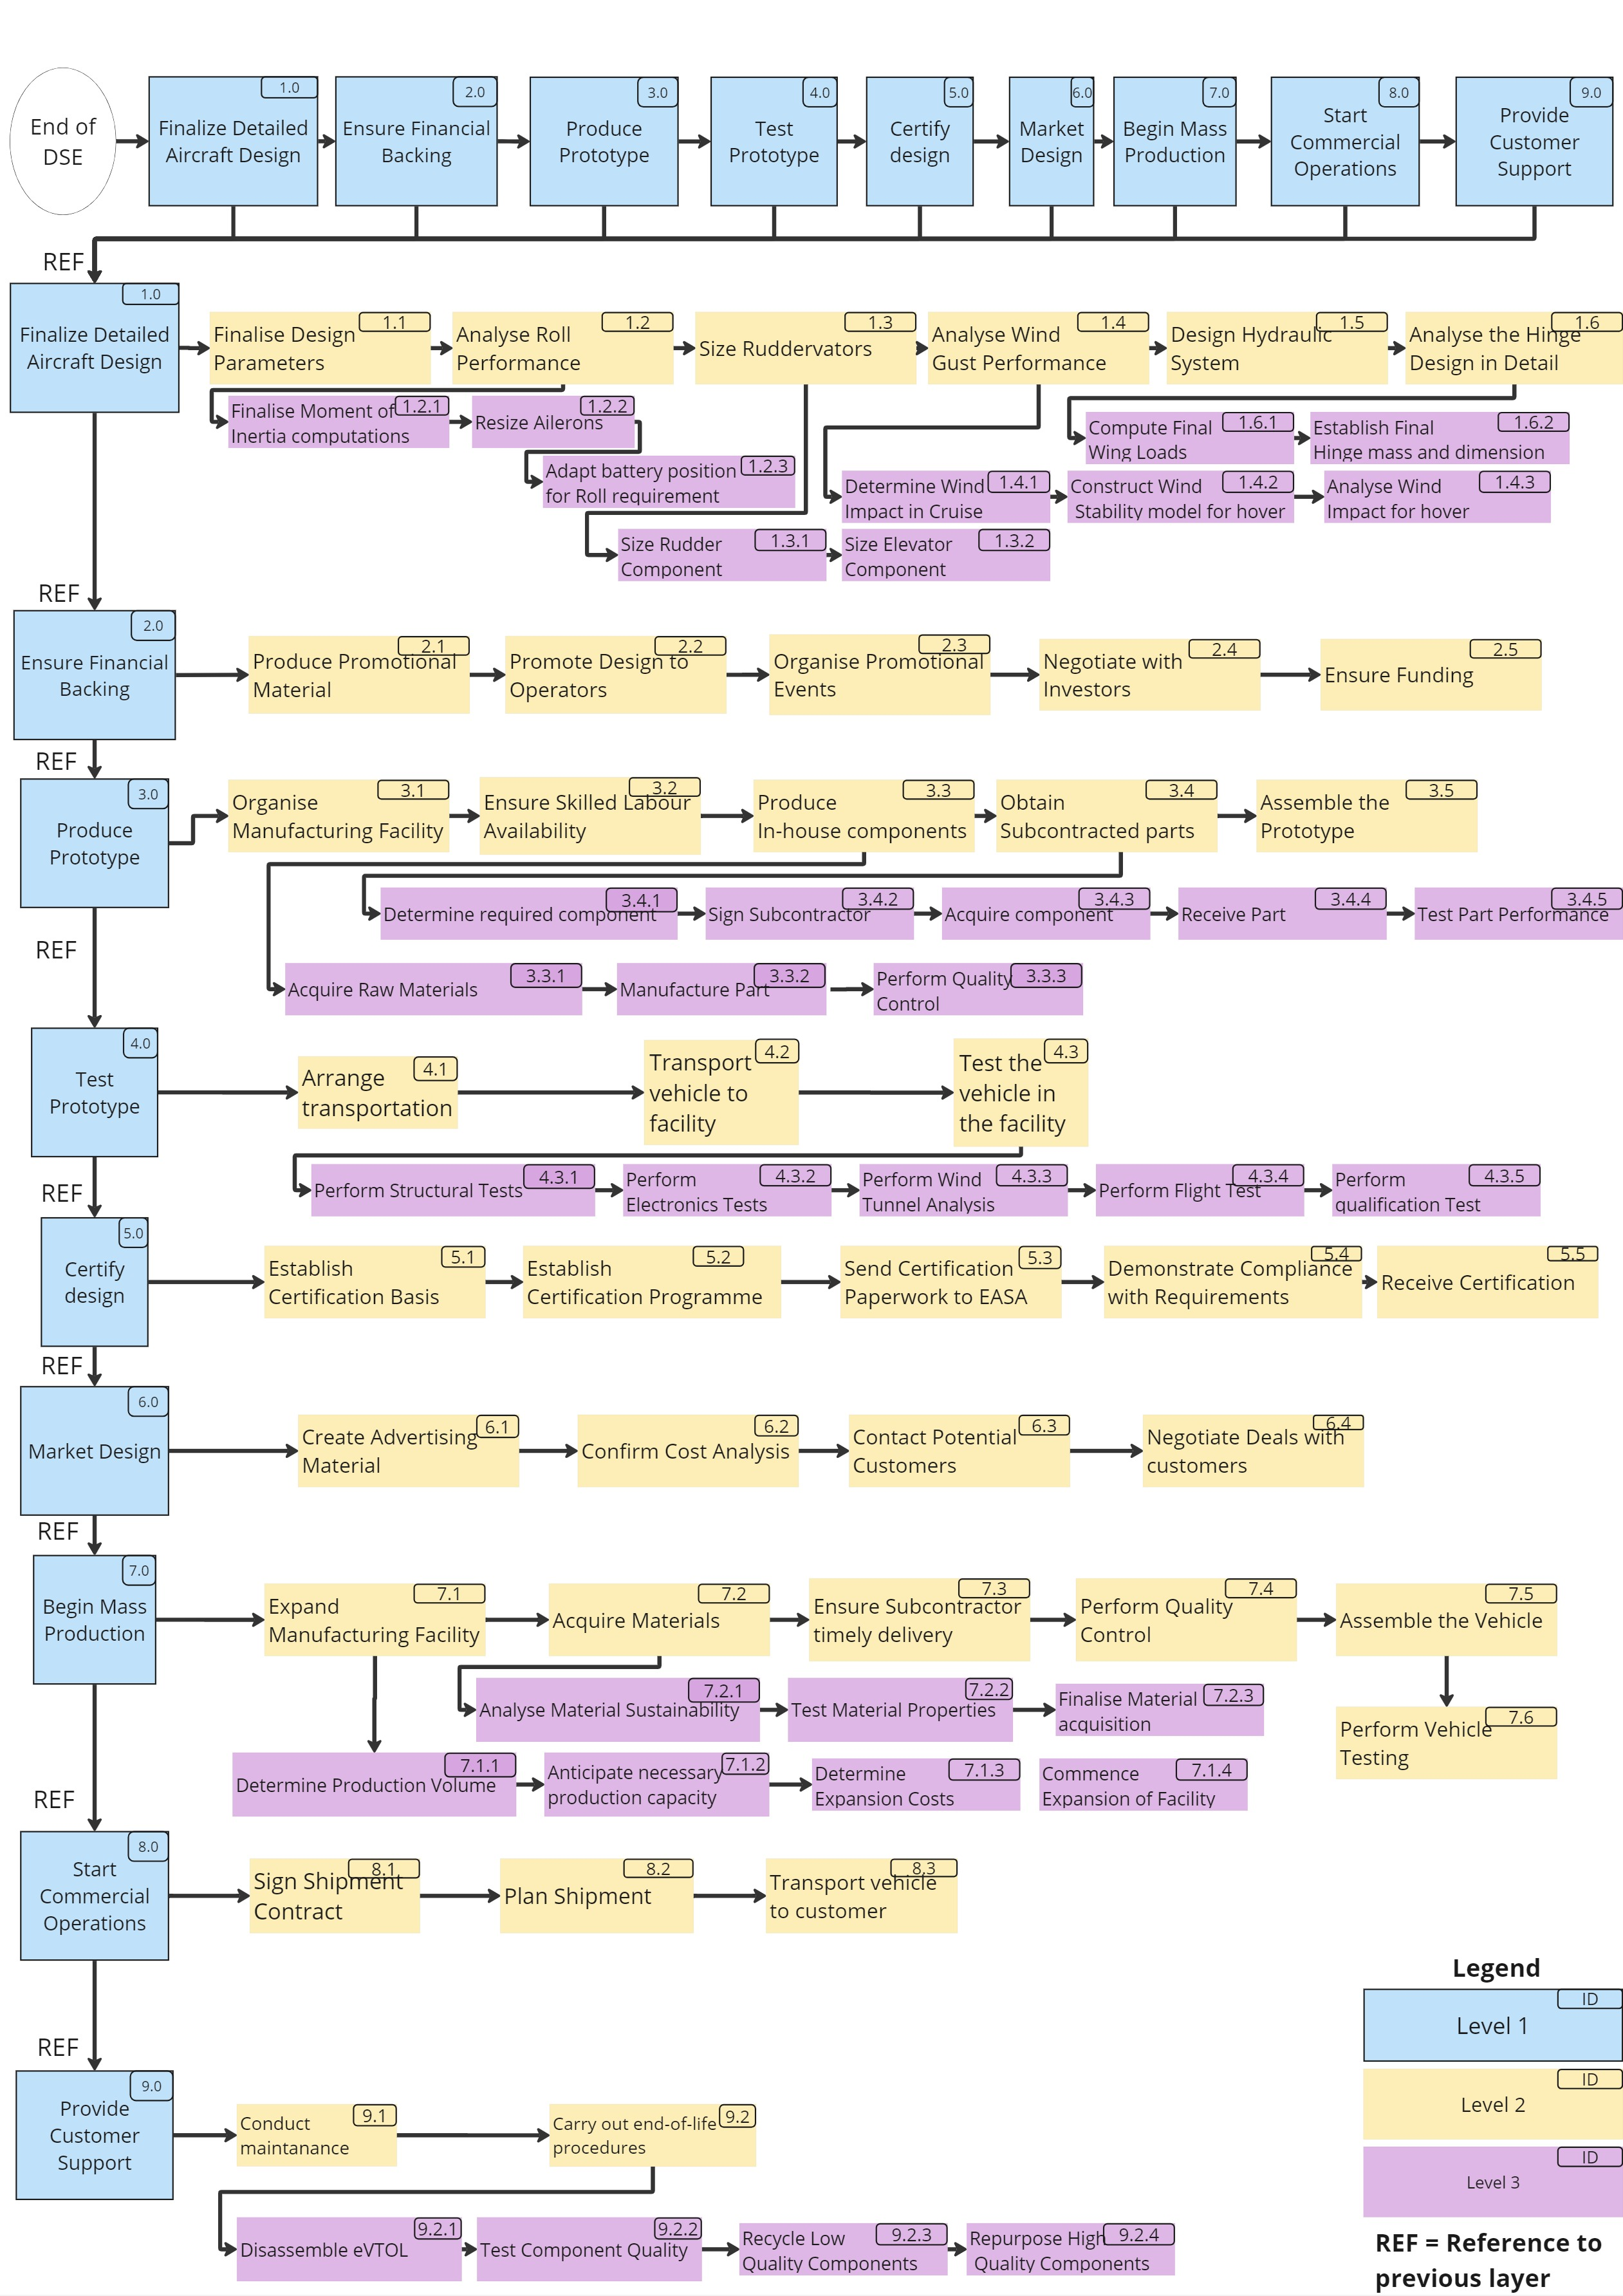
\includegraphics[width=\textwidth]{figures/Project logic}
    \caption{Project logic diagram}
    \label{fig:dev_logic}
\end{figure}

